\documentclass[10pt,reqno]{amsart}
\usepackage{enumerate,amssymb,amsthm}
\usepackage{amsmath,amscd}
\usepackage{tikz}
\usetikzlibrary{decorations.markings,arrows,arrows.meta,cd,calc,decorations.pathmorphing,decorations.pathreplacing,backgrounds,
positioning,fit,snakes}
\tikzset{snake it/.style={decorate, decoration={snake, segment length=3mm, amplitude=0.5mm}}}

\begin{document}

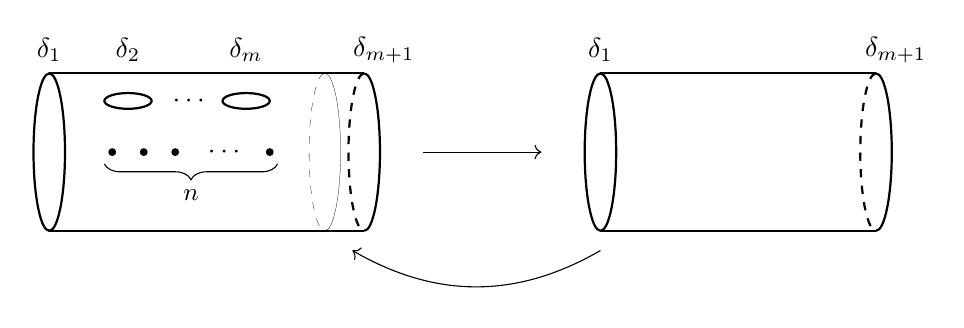
\begin{tikzpicture}[thick]
  % Left main cylinder: outer ellipses and horizontal lines
  \draw (0,0) ellipse (0.2cm and 1cm);
  \draw (0,1) -- (4,1);
  \draw (0,-1) -- (4,-1);
  \draw[dashed] (4,1) arc (90:270:0.2cm and 1cm);
  \draw (4,1) arc (90:-90:0.2cm and 1cm);

  % Internal small ellipses and dots inside the left cylinder
  \draw (1,0.65) ellipse (0.3cm and 0.1cm);
  \draw (2.5,0.65) ellipse (0.3cm and 0.1cm);
  \draw (1.8,0.65) node {$\cdots$};
  \fill (0.8,0) circle (0.05);
  \fill (1.2,0) circle (0.05);
  \fill (1.6,0) circle (0.05);
  \fill (2.8,0) circle (0.05);
  \draw (2.25,0) node {$\cdots$};

  % Labels above the left cylinder
  \draw (0,1.3) node {$\delta_1$};
  \draw (1,1.3) node {$\delta_2$};
  \draw (2.5,1.3) node {$\delta_m$};
  \draw (4.25,1.3) node {$\delta_{m+1}$};

  % Brace with label below the dots
  \draw [thin, snake=brace, segment amplitude=2mm] (2.9,-0.15) -- (0.7,-0.15);
  \draw (1.8,-0.55) node {\small$n$};

  % Additional internal cylinder (dashed/solid arcs) near the right end of left diagram
  \begin{scope}[ultra thin]
    \draw[dashed] (3.5,1) arc (90:270:0.2cm and 1cm);
    \draw (3.5,1) arc (90:-90:0.2cm and 1cm);
  \end{scope}

  % Arrows connecting left and right diagrams
  \draw[thin, ->] (4.75,0) -- (6.25,0);
  \draw[thin, ->] (7,-1.25) to [bend left] (3.85,-1.25);

  % Right diagram (shifted by 7cm)
  \begin{scope}[xshift=7cm]
    % Main cylinder structure
    \draw (0,0) ellipse (0.2cm and 1cm);
    \draw (0,1) -- (3.5,1);
    \draw (0,-1) -- (3.5,-1);
    \draw[dashed] (3.5,1) arc (90:270:0.2cm and 1cm);
    \draw (3.5,1) arc (90:-90:0.2cm and 1cm);
    % Labels
    \draw (0,1.3) node {$\delta_1$};
    \draw (3.75,1.3) node {$\delta_{m+1}$};
  \end{scope}
\end{tikzpicture}

\end{document}